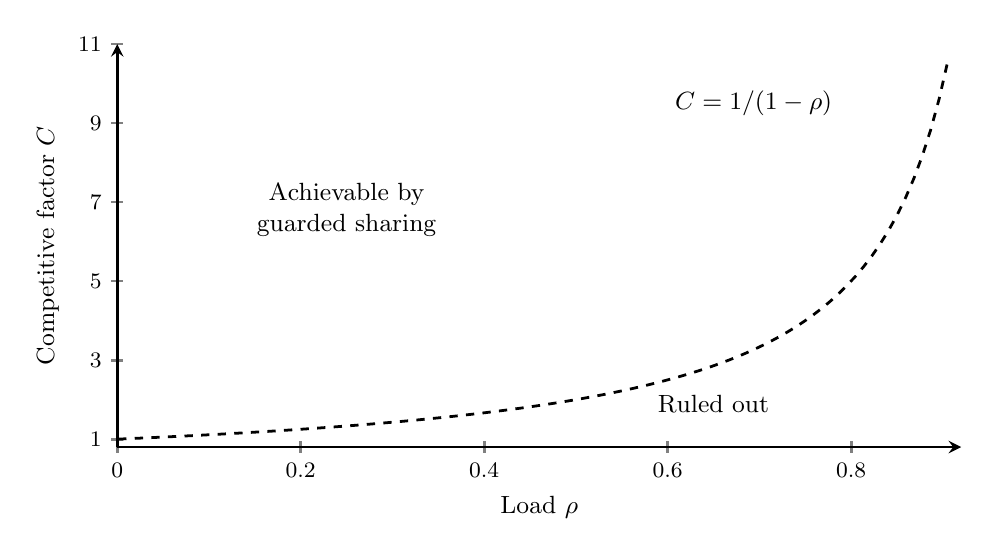
\begin{tikzpicture}
\begin{axis}[
 width=12.3cm,height=6.7cm,
 xmin=0,xmax=.92,ymin=.8,ymax=11,
 xlabel={Load $\rho$},ylabel={Competitive factor $C$},
 xtick={0,.2,.4,.6,.8},ytick={1,3,5,7,9,11},
 axis lines=left,clip=true,
 axis line style={line width=1pt},tick style={line width=1pt},
 tick label style={font=\footnotesize},
 label style={font=\small}]
 \addplot[black,dashed,line width=1pt,domain=.001:.905,samples=100] {1/(1-x)};
 \node[align=center,font=\small] at (axis cs:.25,6.8)
   {Achievable by\\guarded sharing};
 \node[align=center,font=\small] at (axis cs:.65,1.9)
   {Ruled out};
 \node[anchor=east,font=\small] at (axis cs:.79,9.5)
   {$C=1/(1-\rho)$};
\end{axis}
\end{tikzpicture}
